% Architecture section for AgriConnect documentation
\section{System Architecture}

\subsection{Architecture Overview}
AgriConnect follows a three-tier client-server architecture:
\begin{itemize}[leftmargin=*]
	\item \textbf{Client Tier}: Next.js frontend.
	\item \textbf{Server Tier}: Django backend API.
	\item \textbf{Data Tier}: PostgreSQL database.
\end{itemize}

\begin{figure}[H]
	\centering
	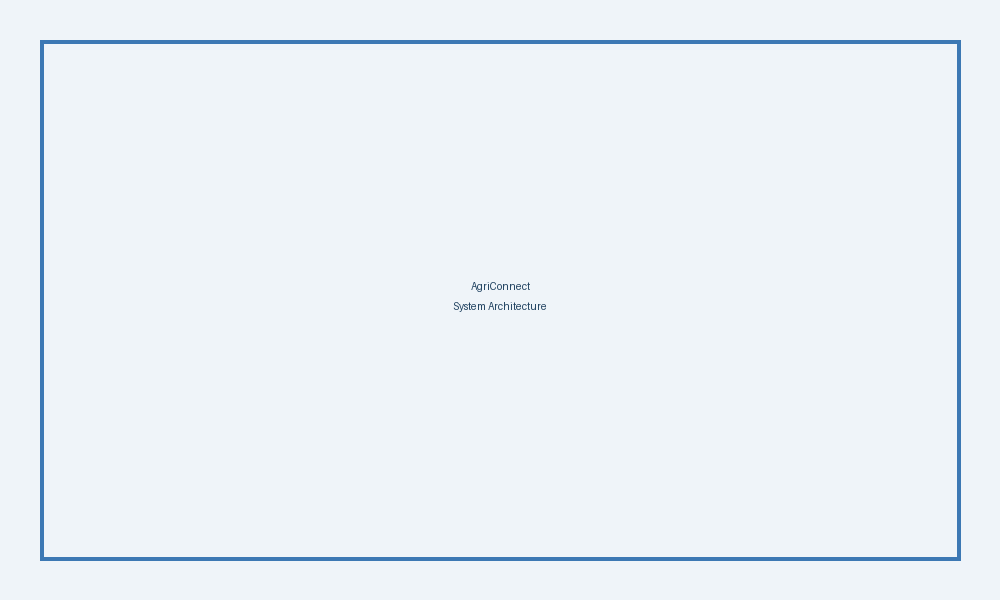
\includegraphics[width=0.8\textwidth]{images/architecture.png}
	\caption{System Architecture Diagram}
	\label{fig:architecture}
\end{figure}

\subsection{Client Tier}
The frontend is built with Next.js 13 and TypeScript:
\begin{itemize}[leftmargin=*]
	\item Uses the App Router for routing pages.
	\item React components render the UI.
	\item Tailwind CSS handles styling.
	\item Axios manages API calls.
\end{itemize}

\subsection{Server Tier}
The backend uses Django REST Framework:
\begin{itemize}[leftmargin=*]
	\item Provides RESTful API endpoints.
	\item Implements JWT authentication.
	\item Persists data via PostgreSQL using the Django ORM.
	\item Leverages Redis for caching.
\end{itemize}

\subsection{Data Flow}
\begin{enumerate}[leftmargin=*]
	\item The user interacts with the Next.js frontend.
	\item The frontend issues requests to the Django API.
	\item Django processes the request and queries PostgreSQL.
	\item The response returns to the frontend.
	\item The UI updates and presents the data to the user.
\end{enumerate}
